\documentclass[a4paper,12pt]{report}
\usepackage[utf8]{inputenc}
\usepackage{geometry}

 \geometry{
  top=2cm,
	bottom=2cm,
	left=2.5cm,
	right=2cm,	
	 headheight=17pt, % as per the warning by fancyhdr
	includehead,includefoot,
	heightrounded, %
}

%misselanious
\usepackage[parfill]{parskip}
\usepackage{url}
\usepackage{float}

%language
\usepackage[english,german]{babel}
% last listed language is selected by default
%use \selectlanguage{<language>} to switch language within the document

%pictures
\usepackage{graphicx}
\graphicspath{ {pics/} }

%header & footer
\usepackage{lastpage}
\usepackage{fancyhdr}


\pagestyle{fancy}
	\fancyhf{}
	\lhead{\slshape \leftmark}
	\rhead{Softwareentwicklungsprozesse}
	\renewcommand{\chaptermark}[1]{ \markboth{#1}{} }
	\rfoot{\thepage{ }/ \pageref{LastPage}}
%\pagestyle{fancy}



%title formating of report class
\usepackage{titlesec}
\titleformat{\chapter}{\normalfont\huge}{\thechapter.}{20pt}{\huge}

%bibliography
\usepackage{cite}



\begin{document}	

\begin{titlepage}
\begin{center}
  
\includegraphics[scale=0.6]{FHNW-LOGO.png}
  \vskip.2in
  \textsc{\LARGE Software-Entwicklungsprozesse}
  \vskip.2in
  \Large Aufgabe 2.2 
  \vskip1in
  \emph{\huge Gegenüberstellung Scrum - DAD}
  \vskip1.4in
  \bfseries
  \today
\end{center}

\vskip1in

\begin{minipage}[t]{.25\textwidth}
  \begin{flushleft}
    \bfseries\large Dozentin:\par 
    \emph{Sybille Peter}
  \end{flushleft}
\end{minipage}
\hskip.4\textwidth
\begin{minipage}[t]{.5\textwidth}
  \begin{flushleft}
    \bfseries\large Studenten:\par
    \emph{Eggenschwiler Carlo}\newline
    \emph{Frei Dominik}\newline
    \emph{Frommwiler Dominic}\newline
    \emph{Inniger Marco}
  \end{flushleft}
\end{minipage}


\end{titlepage}

\pagenumbering{arabic}

\chapter*{Zusammenfassung}
\thispagestyle{fancy}

Diese Arbeit liefert eine Gegenüberstellung von Scrum und Disciplined Agile Delivery. Der Fokus wird auf die Themen Planung, Zusammenarbeit und Zuständigkeit gelegt. Es werden Grundkenntnisse über das Vorgehensmodell Scrum oder Extrem Programming (XP) vorausgesetzt.

Disciplined Agile Delivery (DAD) basiert grösstenteils auf Scrum und Extreme Programming. Im Zentrum steht die Construction Phase mit Iterationen (Sprints) von fixer Zeitdauer. Dieses Vorgehensmodel findet dann Anwendung, wenn Scrum den Bedürfnissen nicht mehr genügt und erweitert werden muss und ein agiles Projekt durchgeführt werden muss.

DAD ist \textbf{iterationsbasiert}. Wie bei vielen agilen Methoden, einschliesslich Scrum und XP, wird die Lösung schrittweise und zeitgesteuert aufgebaut. Diese Zeitrahmen werden Iterationen genannt (was Scrum Sprints nennt).

DAD verwendet \textbf{nicht die Scrum Terminologie}. Die Entwickler von DAD haben sich explizit gegen die Scrum Terminologie entschieden. Jedoch spielt diese keine Rolle. So darf in DAD mit der Scrum Terminologie gearbeitet werden.

DAD zeigt \textbf{Eingaben von ausserhalb des Lieferlebenszyklus} auf. DAD zeigt, dass vor Beginn des Projekts etwas passiert und dass agile Teams oft neue Anforderungen (in Form von Änderungsanfragen und Fehlermeldungen) aus der Produktion erhalten. Diese Inputs liefern einen wichtigen Kontext für den gesamten Lieferlebenszyklus.

Es gibt eine \textbf{Workitem-Liste} und kein Product Backlog. DAD hat einen grösseren Umfang als Scrum, und wenn man diesen grösseren Umfang berücksichtigt, beginnt man zu erkennen, dass man einen robusteren Change Management-Ansatz benötigt als den Product Backlog von Scrum. Zu den Workitems gehören Anforderungen, Mängel und andere nicht funktionalitätsorientierte Arbeiten wie Schulungen, Ferien und die Unterstützung anderer Teams. Alle diese Arbeiten müssen irgendwie priorisiert werden, nicht nur die Umsetzung der Anforderungen.

Es enthält \textbf{explizite Meilensteine}. Am Ende des Lebenszyklusdiagramms finden sich Hinweise auf vorgeschlagene leichte Meilensteine, die von den Lieferteams angestrebt werden sollten. Solche Meilensteine sind ein wichtiger Aspekt agiler Governance.

\pagebreak
DAD sollte in folgdenden Fällen angewendet werden:

\begin{itemize}
	\item Die Arbeit kann frühzeitig im Projekt identifiziert, priorisiert und geschätzt werden.
	\item Eine gute Wahl für neue agile Teams.
	\item Das Team ist mit Scrum und XP vertraut.
	\item Das Team arbeitet typischerweise an einem Projekt.
\end{itemize}



\tableofcontents
\thispagestyle{fancy}


\chapter{Einführung}
\thispagestyle{fancy}
Diese Arbeit zeigt auf wie DAD auf Scrum angewendet wird und welchen Mehrwert dadurch gewonnen wird. Wir fokussieren uns explizit in dieser Arbeit nur auf Scrum, da ein Vergleich mit allen agilen Methoden nicht umsetzbar gewesen ist. Zudem ist durch den Auftrag gegeben, dass Scrum vom bestehenden Team bereits angewendet wird.
Wir empfehlen jedoch als zusätzliche Quelle das Buch «Choose your WoW! A Disciplined Agie Delivery Handbook for Optimizing Your Way of Working» \cite{dadHandbook}.

\section{Was ist Disciplined Agile Delivery?}

Disciplined Agile Delivery (DAD) ist ein Hybrid-Prozess beziehungsweise ein Framework, welches agile Vorgehensmodelle, wie beispielsweise Scrum, integriert. Die Erfinder von DAD (Scott Ambler und Mark Lines) sehen agile Prozesse als nicht voll umfänglich. Scrum beantwortet viele Fragen nicht, welche sich stellen, wenn das Modell in einem komplexeren Umfeld angewendet wird. DAD bietet zusätzliche Fragestellungen und Methoden um gerade komplexe Strukturen auf einen agilen Pfad zu bringen. DAD ist somit eine Ergänzung zu den agilen Vorgehensweisen wie Scrum, Extreme Programming, Kanban, Lean, etc. DAD ermöglicht bestehende agile Prozesse auf komplexere Unternehmenstrukturen anzuwenden.\newline

\begin{figure}[H]
	\centering
	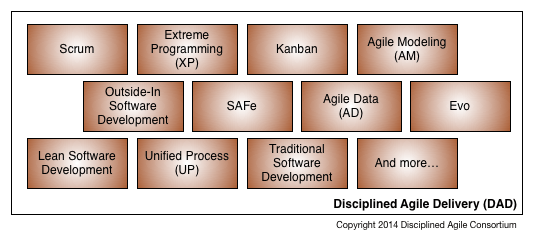
\includegraphics[scale=0.8]{hybrid1}
	\caption{DAD als hybrides Vorgehensmodell \cite{dadHybrid}}
	\label{fig:hybrid}
\end{figure}
\subsection{Phasen in DAD}
Allgemein kann gesagt werden, dass DAD aus drei Phasen besteht: Inception, Construction und Transition (Abbildung \ref{fig:highlevellifecycle}). \smallskip
\begin{figure}[H]
	\centering
	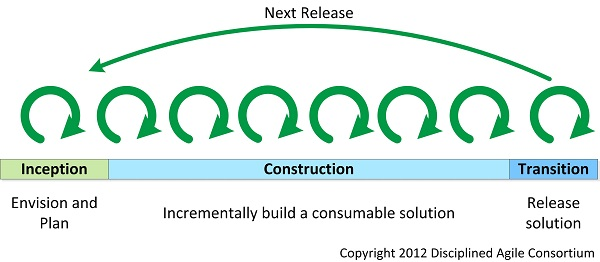
\includegraphics[width=\textwidth]{lifecycle}
	\caption{Highlevel Lifecycle von DAD\cite{lifecycleDAD}}
	\label{fig:highlevellifecycle}
\end{figure}\medskip
In der \textbf{Inception} Phase wird die Planung und Analyse des Projekts und dessen Ressourcen gemacht. Dies umfasst folgende Schritte:\smallskip
\begin{itemize}
	\item Initiales Team bilden
	\item Projekt Vision identifizieren
	\item Mit Stakeholder auf die Projekt-Vision einigen
	\item Auf Unternehmensstrategie abstimmen
	\item Technische Strategie, initiale Anforderungen und initiale Release-Planung festlegen
	\item Arbeitsumfeld einrichten
	\item Finanzierung sichern
	\item Risiken identifizieren
\end{itemize}
\medskip
Die \textbf{Construction} Phase beinhaltet die eigentliche Entwicklung und das Testen, wo das entsprechende Vorgehensmodell eingesetzt wird. Sie umfasst folgende Punkte:\smallskip
\begin{itemize}
	\item Eine verwendbare Lösung liefern
	\item Ändernde Bedürfnisse der Stakeholder adressieren 
	\item Näher an das einsetzbare Produkt herankommen
	\item Qualität verbessern oder höhere Qualität erarbeiten
	\item Architektur frühzeitig beweisen
	\item Arbeitsumfeld einrichten
\end{itemize}\medskip
Die \textbf{Transition} Phase betrifft Zieleinhaltung und Lieferung. Folgende Punkte gehören zu dieser Phase:
\begin{itemize}
	\item Einsatzfähigkeit der Lösung sicherstellen
	\item Empfangsbereitschaft der Stakeholder sicherstellen
	\item Lösung in produktive Umgebung liefern
\end{itemize}
\medskip

Auffallend ist hier, dass die Phasen identisch mit jenen von RUP (Rational Unified Process) sind\cite{rup}. DAD beinhaltet als nebst den Fundamenten von Scrum und XP auch jene von RUP.


\subsection{DAD als Scrum-basiertes Vorgehensmodell}

DAD als agiles Vorgehensmodell bedeutet eine erweiterte Scrum Vorgehensweise. Scrum wird dort erweitert wo es unzureichend definiert ist. In Abbildung \ref{fig:lifecycle} ist der komplette Lifecycle des Scrum-basierten DAD dargestellt. Diese Abbildung scheint auf den ersten Blick sehr komplex. Bei genauerer Betrachtung ist aber ersichtlich, dass der Lifecycle viele Gemeinsamkeiten mit jenem von Scrum hat.


\begin{figure}[H]
	\centering
	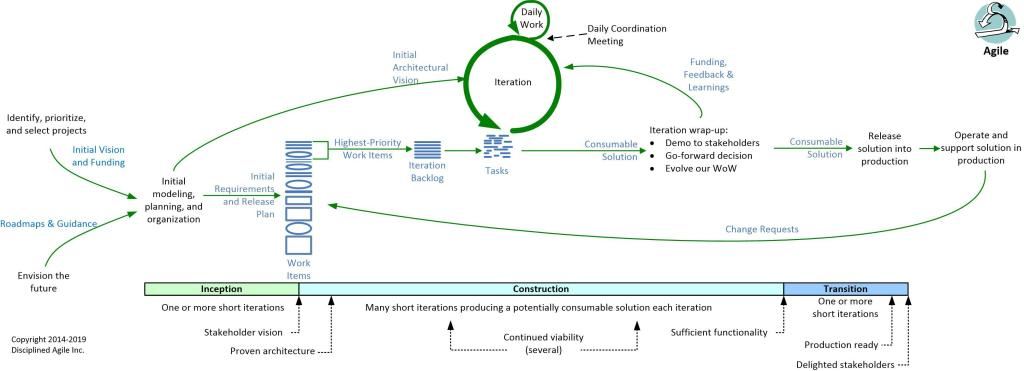
\includegraphics[width=\textwidth]{Lifecycle-DAD-Agile}
	\caption{Scrum-basiertes DAD Vorgehensmodells \cite{lifecycleDAD}}
	\label{fig:lifecycle}
\end{figure}\medskip

Dieses Vorgehensmodell bietet folgende interessante Aspekte:
\begin{itemize}
	\item Es ist iterationsbasiert.
	\item Es verwendet keine Scrum-Terminologie.
	\item Es zeigt Inputs ausserhalb des Vorgehensmodelles an.
	\item Es gibt eine Workitem-Liste, kein Product Backlog.
	\item Es enthält explizite Meilensteine.
\end{itemize}

\section{Anwendungsgebiete der beiden\newline Vorgehensmodelle}

Scrum wird häufig im Kontext von IT, Software-Entwicklung, Design oder Marketing oder kontextähnlichen Gebieten eingesetzt. Jedoch ist wichtig, dass Scrum in allen Branchen zur Anwendung kommt.

DAD kann im selben Kontext wie Scrum genutzt werden. Jedoch ist die Anwendung nur in komplexeren Unternehmenstrukturen sinnvoll. Zudem ist DAD geeignet als Mittel zur Transition von hierarchisch geprägten Strukturen zu agilen, selbstständigen Teams.
 



\chapter{Gegenüberstellung}
\thispagestyle{fancy}
\section{Planung}

Das Thema Planung wird unter folgenden fünf Aspekten betrachtet:
\begin{enumerate}
\item Release-Planung
\item Priorisierung
\item Planungssicherheit
\item Planungsaufwands
\item Nachvollziehbarkeit
\end{enumerate}

\subsection{Release-Planung}

{\Large Scrum:} \cite{planningReleaseScrum} \medskip

Der Release-Plan ist ein höhergestellter Plan, der mehrere Sprints beinhaltet und während der Release-Planung festgelegt wird. Der Plan definiert welche Features umgesetzt werden und wann diese erfüllt sind. Er dient auch dazu, den Fortschritt innerhalb des Projekts verfolgen zu können. Es können mehrere Releases während des Projekts geplant werden, oder einfach ein finales Release am Ende des Projekts. \medskip

Um eine Release-Planung durchführen zu können muss folgendes bekannt sein:
\begin{itemize}
\item Ein priorisiertes Scrum-Backlog
\item Die Ressourcen des Scrum-Teams
\item Zielerfüllungsbedingungen
\end{itemize}
Ein Release-Plan kann Termin- oder Feature-geführt sein.\smallskip

Bei Termin-geführten Projekten wird spezifiziert, welche Features bis zu einem bestimmten Termin erfüllt werden können.\smallskip

Bei Feature-geführten Projekten wird spezifiziert , bis zu welchem Termin das Features erfüllt ist.\smallskip

Wie der Backlog ist auch der Release-Plan bei Scrum nicht statisch. Dieser kann sich mit dem Backlog ändern oder auch nach jedem Sprint wieder diskutiert und überarbeitet werden.
\bigskip 

{\Large DAD:} \cite{planningReleaseDad} \medskip

In DAD wird die Release Planung initial in der Inception Phase gemacht. Der Leitfaden empfiehlt für die Releaseplanung folgende sechs Fragen zu beantworten.
\begin{itemize}
	\item Wer wird an der Planung beteiligt sein?
	\item Was ist der Umfang unseres Planungsaufwands?
	\item Was ist unsere Gesamtstrategie, die diesen Plan vorantreibt?
    \item Wie detailliert sollte unser Plan sein?
    \item Welche Kadenzen wird das Team annehmen?
    \item Welchen Ansatz zur Schätzung werden wir wählen?
\end{itemize}
Damit soll sichergestellt werden, dass grundlegende Managementfragen gegenüber den Stakeholder beantwortet sind. Zudem wird erreicht, dass eine durchführbare Strategie besteht und zwischen Stakeholder und Delivery Team ein gemeinsames Verständnis existiert.


\subsection{Priorisierung}

{\Large Scrum:} \cite{planningPrioScrum} \medskip

Das Scrum-Team priorisiert zusammen mit dem Product-Owner die Tasks/Stories aus dem Scrum-Backlog. Wichtig dabei ist, dass nicht nur priorisiert, sondern dass auch sortiert werden muss. Beim Sortieren wird auch die Reihenfolge von Abläufen berücksichtigt. Die Priorisierung geht mit der Sortierung Hand in Hand. \smallskip

Weiter achtet Scrum auch darauf, dass die wertvollsten Inkremente frühstmöglich umgesetzt werden.\bigskip 

{\Large DAD:} \cite{planningPrioDad} \medskip

Die Priorisierung bei DAD verhält sich ähnlich wie die Release-Planung. Grundsätzlich gilt wieder das Rolling-Wave-Modell. Dass heisst, dass höher priorisierte Features detaillierter spezifiziert werden und tief priorisierte nur grob. Die Priorisierung kann jederzeit wieder angepasst werden.


\subsection{Planungsumfang}

{\Large Scrum:} \medskip

In Scrum betrifft der Umfang immer direkt das Produkt. Der Scope beinhaltet Features ausgedrückt z.B. als User Stories. Diese sind im Scrum-Backlog abgelegt und verwaltet.
\bigskip 

{\Large DAD:} \cite{planningScopeDad} \medskip

DAD geht hier einen Schritt weiter und definiert nicht nur Features sondern sogenannte Working-Items. Bei denen werden auch nicht-funktionale Anforderungen definiert wie z.B. Schulungen, Ferien, Unterstützung anderer Teams usw.	


\subsection{Planungsaufwand}

{\Large Scrum:} \medskip

Der Planungsaufwand von Scrum ist relativ gering und ist eigentlich im iterierenden Prozess von Scrum bereits integriert. Die Planung wird bei Scrum vor jedem Sprint im sogenannten Sprint Planning gemacht. Dabei werden die zu erledigenden Items definiert. Der Umfang des Sprints wird vom ganzen Team bestätigt.\bigskip 

{\Large DAD:} \medskip

Initial ist der Planungsaufwand bei DAD hoch. Man muss nebst der eigentlichen Planung des Produkts auch diverse Analysen von Ist-Zuständen bezüglich Ressourcen und Zuständen innerhalb des Unternehmens machen um die Rahmenbedingungen für das Projekt zu legen. Während der Construction Phase ist der Planungsaufwand analog demjenigen von Scrum.


\subsection{Risikomanagement}

{\Large Scrum:} \medskip

Bei Scrum wird das Risikomanagement hauptsächlich durch die Kommunikation zwischen dem Kunden und Team geführt. Diese geht über den Product Owner. Dabei muss der Kunde durch seinen stetigen Einfluss mögliche Risiken ausschliessen können. Er kann dies mittels Akzeptanzkriterien beeinflussen.\newline
Aus teaminterner Sicht ist die Definition of Done das Kontrollinstrument um Qualität aber auch Vollständigkeit sicherzustellen.
Als weiteres Instrument dient die Reviews am Ende jedes Sprints. An jener wird dem Kunde die umgesetzten Items präsentiert. Hier kann der Kunde oder der Product Owner Einfluss bzw. Missverständnisse aufdecken und klären.

\bigskip 

{\Large DAD:} \medskip

Um das Risiko von Fehlkommunikation zu verringern werden bei DAD gegenüber Scrum leichte Meilensteine eingeführt, bei denen ein Abgleich mit dem Kunden stattfindet. \medskip

Weiter sieht DAD die Planung von festen Releases vor. Damit soll regelmässig Software zur Verfügung gestellt werden um ein Feedback des Kunden zu erhalten und frühzeitig festzustellen, ob man die Anforderungen so erfüllen kann. Dies ist gleich wie bei Scrum.

\section{Zuständigkeit und Zusammenarbeit}
\subsection{Rollen}
{\Large Scrum:} \medskip
{\Large DAD:} \medskip


\section{Empfehlung}

Grundsätzlich wäre der Ansatz mit DAD sicher spannend. Ihr Team kann nach wie vor mit Scrum arbeiten und Sie haben die Möglichkeit mit den erwähnten Instrumenten wie leichte Meilensteine, Release Planung der agilen Entwicklung Einfluss zu nehmen und dem ganzen einen ein Rahmen zu geben. \newline
Jedoch wird Sie das Einführen dieses Vorgehensmodell hohen Aufwand kosten. Vor allem muss für das saubere Anwenden von DAD viel Analyse von bestehenden Prozessen und Zuständen innerhalb Ihres Unternehmens betrieben werden.



	

\chapter{Gegenüberstellung Zusammenarbeit}
\thispagestyle{fancy}
\section{Zusammenarbeit}

Das Thema Zuständigkeit wird unter folgenden fünf Aspekten betrachtet:
\begin{enumerate}
\item 	Koordination im Team 
\item 	Rolle und Aufgaben des Kunden \smallskip
		Da in linearen Vorgehensmodellen der Kunde nur an bestimmten Meilensteinen beteiligt ist, interessiert es zu betrachten welche Aufgaben der Kunde hier hat.
\end{enumerate}


\subsection{Koordination im Team}

{\Large Scrum:} \cite{planningReleaseScrum} \medskip

Scrum geht grundsätzlich von einer selbstorganisierenden Koordination aus. Einzig der Scrum Master hat eine "koordinierende" Rolle, jedoch nur im Bezug auf den Prozess und Schnittstellen ausserhalb des Projekts.
Als wichtigstes Instrument für Koordination in Scrum oder auch allgemein in agilen Vorgehensmodellen ist die Kommunikation mit den anderen Team-Mitgliedern. Dies wird in Scrum mit regelmässigen Treffen/Aussprachen realisiert. Wie zum Beispiel das Daily Stand-up oder Scrum of Scrums (Team übergreifend), welche speziell für die Koordination angedacht ist. Weiter Routinen wie Daily Scrum oder Reflektion dienen auch der Koordination und deren Verbesserung, auch wenn das nicht primär ihr Ziel ist.
\bigskip 

{\Large DAD:} \cite{planningReleaseDad} \medskip

DAD möchte, dass folgende Fragen bezüglich Koordination in einem Scrum-Team geklärt sind um eine effektive Organisation innerhalb des Teams zu haben.
\begin{itemize}
	\item 	Wie werden Informationen innerhalb des Teams ausgetauscht?
	\item 	Wer darf die vom Team erstellten Artefakte aktualisieren? 
	\item 	Wie werden wir uns innerhalb des Teams koordinieren?
    \item 	Wenn wir Teil eines größeren Teams sind, wie werden wir dann innerhalb dieses Teams koordinieren?
    \item 	Wie werden wir mit Enterprise-/IT-Teams wie Enterprise Architects und Data Managern zusammenarbeiten?
    \item 	Wie werden wir unsere Release-/Einsatzplanung mit dem Rest des Unternehmens koordinieren?
    \item 	Wenn wir geografisch verteilte Teammitglieder haben, wie werden wir dann mit ihnen zusammenarbeiten?
\end{itemize}
Innerhalb des Teams soll also klar definiert sein, mit welchen Routinen (tägliches Treffen, Video-Konferenzen, usw.) Informationen zwischen den Teammitgliedern ausgetauscht werden und welche Tools dazu verwendet werden. Auch soll auch die Zuständigkeit geregelt sein wer die finalen Artefakten verwaltet, das es hier keine Überschneidungen oder Unklarheiten gibt.
\medskip

Weiter müssen gerade bei agilen Teams innerhalb eines Unternehmen auch die Koordination mit anderen Teams/Abteilungen geregelt sein.
\medskip

Was oft vernachlässigt wird, ist die Koordination mit Teammitglieder an anderen geografischen Orten. Der Informationsaustausch wird hier anspruchsvoller, da direkte verbale Kommunikation, welche die effektivste ist, nicht möglich ist.


\subsection{Rolle und Aufgaben des Kunden}

{\Large Scrum:} \cite{planningPrioScrum} \medskip

Der Kunde soll in Scrum während des ganzen Projektes immer involviert sein. Folgende Möglichkeiten gibt es den Kunden zu involvieren:
\begin{itemize}
	\item Der Kunde wird zum im Initial-Meeting mit einladen.
	\item Backlog wird zusammen mit dem Kunden verwaltet.
	\item Der Kunde nimmt auch an Reviews teil, um Arbeiten zu besprechen und als abgeschlossen zu definieren.
\end{itemize}
Durch den konsequenten Miteinbezug des Kunden wird das Risiko vermindert, dass der Kunde nicht zufrieden ist, da er fortlaufend Einfluss nehmen kann und mit seiner Teilnahme auch frühe Schritte/Arbeiten bestätigt.
\bigskip 

{\Large DAD:} \cite{planningPrioDad} \medskip

DAD hat bezüglich dem Kunden eine andere auch radikalere Haltung. In DAD will man den Begriff "Kunde" nicht verwenden, sondern nur Stakeholder. Dieser werden in folgende Gruppen unterteilt:
\begin{itemize}
	\item Endbenutzer: Personen die das Produkt schlussendlich verwenden.
	\item Vorstehende: Personen die schlussendlich entscheiden, welches Produkt beschafft wird, Bezahlungen freigeben, usw. werden
	\item Partner: Unterhalter, Betreiber, Entwickler von externen Systemen, Juristen, usw.
	\item Interne: Personen innerhalb des Entwicklungsteams und welche technische oder geschäftliche Dienste liefern
\end{itemize}
Für ein Produkt gibt es nur Stakeholders und es gilt dessen Anforderung genau zu ermitteln und festzulegen. Dazu werden für alle Stakeholder die Bedürfnisse gleichwertig ermittelt und miteinbezogen. \smallskip

Man will also bewusst ein Produkt, dass alle Stakeholder gleich berücksichtigen und nicht nur den bezahlenden Kunden" hauptsächlich priorisieren. Denn nur so wird der abbezahlende Kunde" auch ein nachhaltiges und erfolgreiches Produkt erhalten können.
\medskip
Als wichtig wird auch herausgehoben, dass das Projekt im "wir"-Kontext betrachtet wird und nicht im "ihr". Es gibt nicht den Kunden und das Entwicklungsteam, sondern das Projekt betrifft alle gleich.


\section{Empfehlung}

Grundsätzlich wäre der Ansatz mit DAD sicher spannend. Ihr Team kann nach wie vor mit Scrum arbeiten und Sie haben die Möglichkeit mit den erwähnten Instrumenten wie leichte Meilensteine, Release Planung der agilen Entwicklung Einfluss zu nehmen und dem ganzen einen ein Rahmen zu geben. \newline
Jedoch wird Sie das Einführen dieses Vorgehensmodell hohen Aufwand kosten. Vor allem muss für das saubere Anwenden von DAD viel Analyse von bestehenden Prozessen und Zuständen innerhalb Ihres Unternehmens betrieben werden.



	

\listoffigures
\thispagestyle{fancy}


\bibliography{main}{}
\bibliographystyle{unsrt}
\thispagestyle{fancy}

\end{document}